\section{Watership Down \& Hot Pants}

\margininbox{Winter Journey}{
     \begin{itemize}
    \item Jarvist Frost
    \item Clare Tan
    \end{itemize}}{\explo}


The camp was set up and exploration was in full swing. The way out East
already had its cohort of converts. For me there was one pushing front
which had primacy above all others -- namely the deepest point in the
cave. \passage{Winter Journey}, which I had explored with Jim and Fratnik
last year, had a few niggling leads but nothing stellar. The silt
deposits and depth indicated that a sump was not far away, but the
inclined bedding heading North could continue for a very long time. With
an interest in diving the sumps, I also had a distinct interest in the
flooded sections.

Luckily Clare was easily suggested with the very bottom as a target. One
concern was that the wet pitch series through \passage{Daydreamers} had been left
rigged last year -- we had anticipated further trips after our last one,
but weather put paid to this. So we took a tackle sac of string to patch
the pitches where necessary.

The one negative point was my little Canon `pocket camera', hauled with
nary a care in a Pelicase through all kinds of horrific caving locations
over the previous six years had finally given up the ghost -- and so we
had no way to photographically record where we were visiting.

\begin{marginfigure}
\checkoddpage \ifoddpage \forcerectofloat \else \forceversofloat \fi
\centering
 \frame{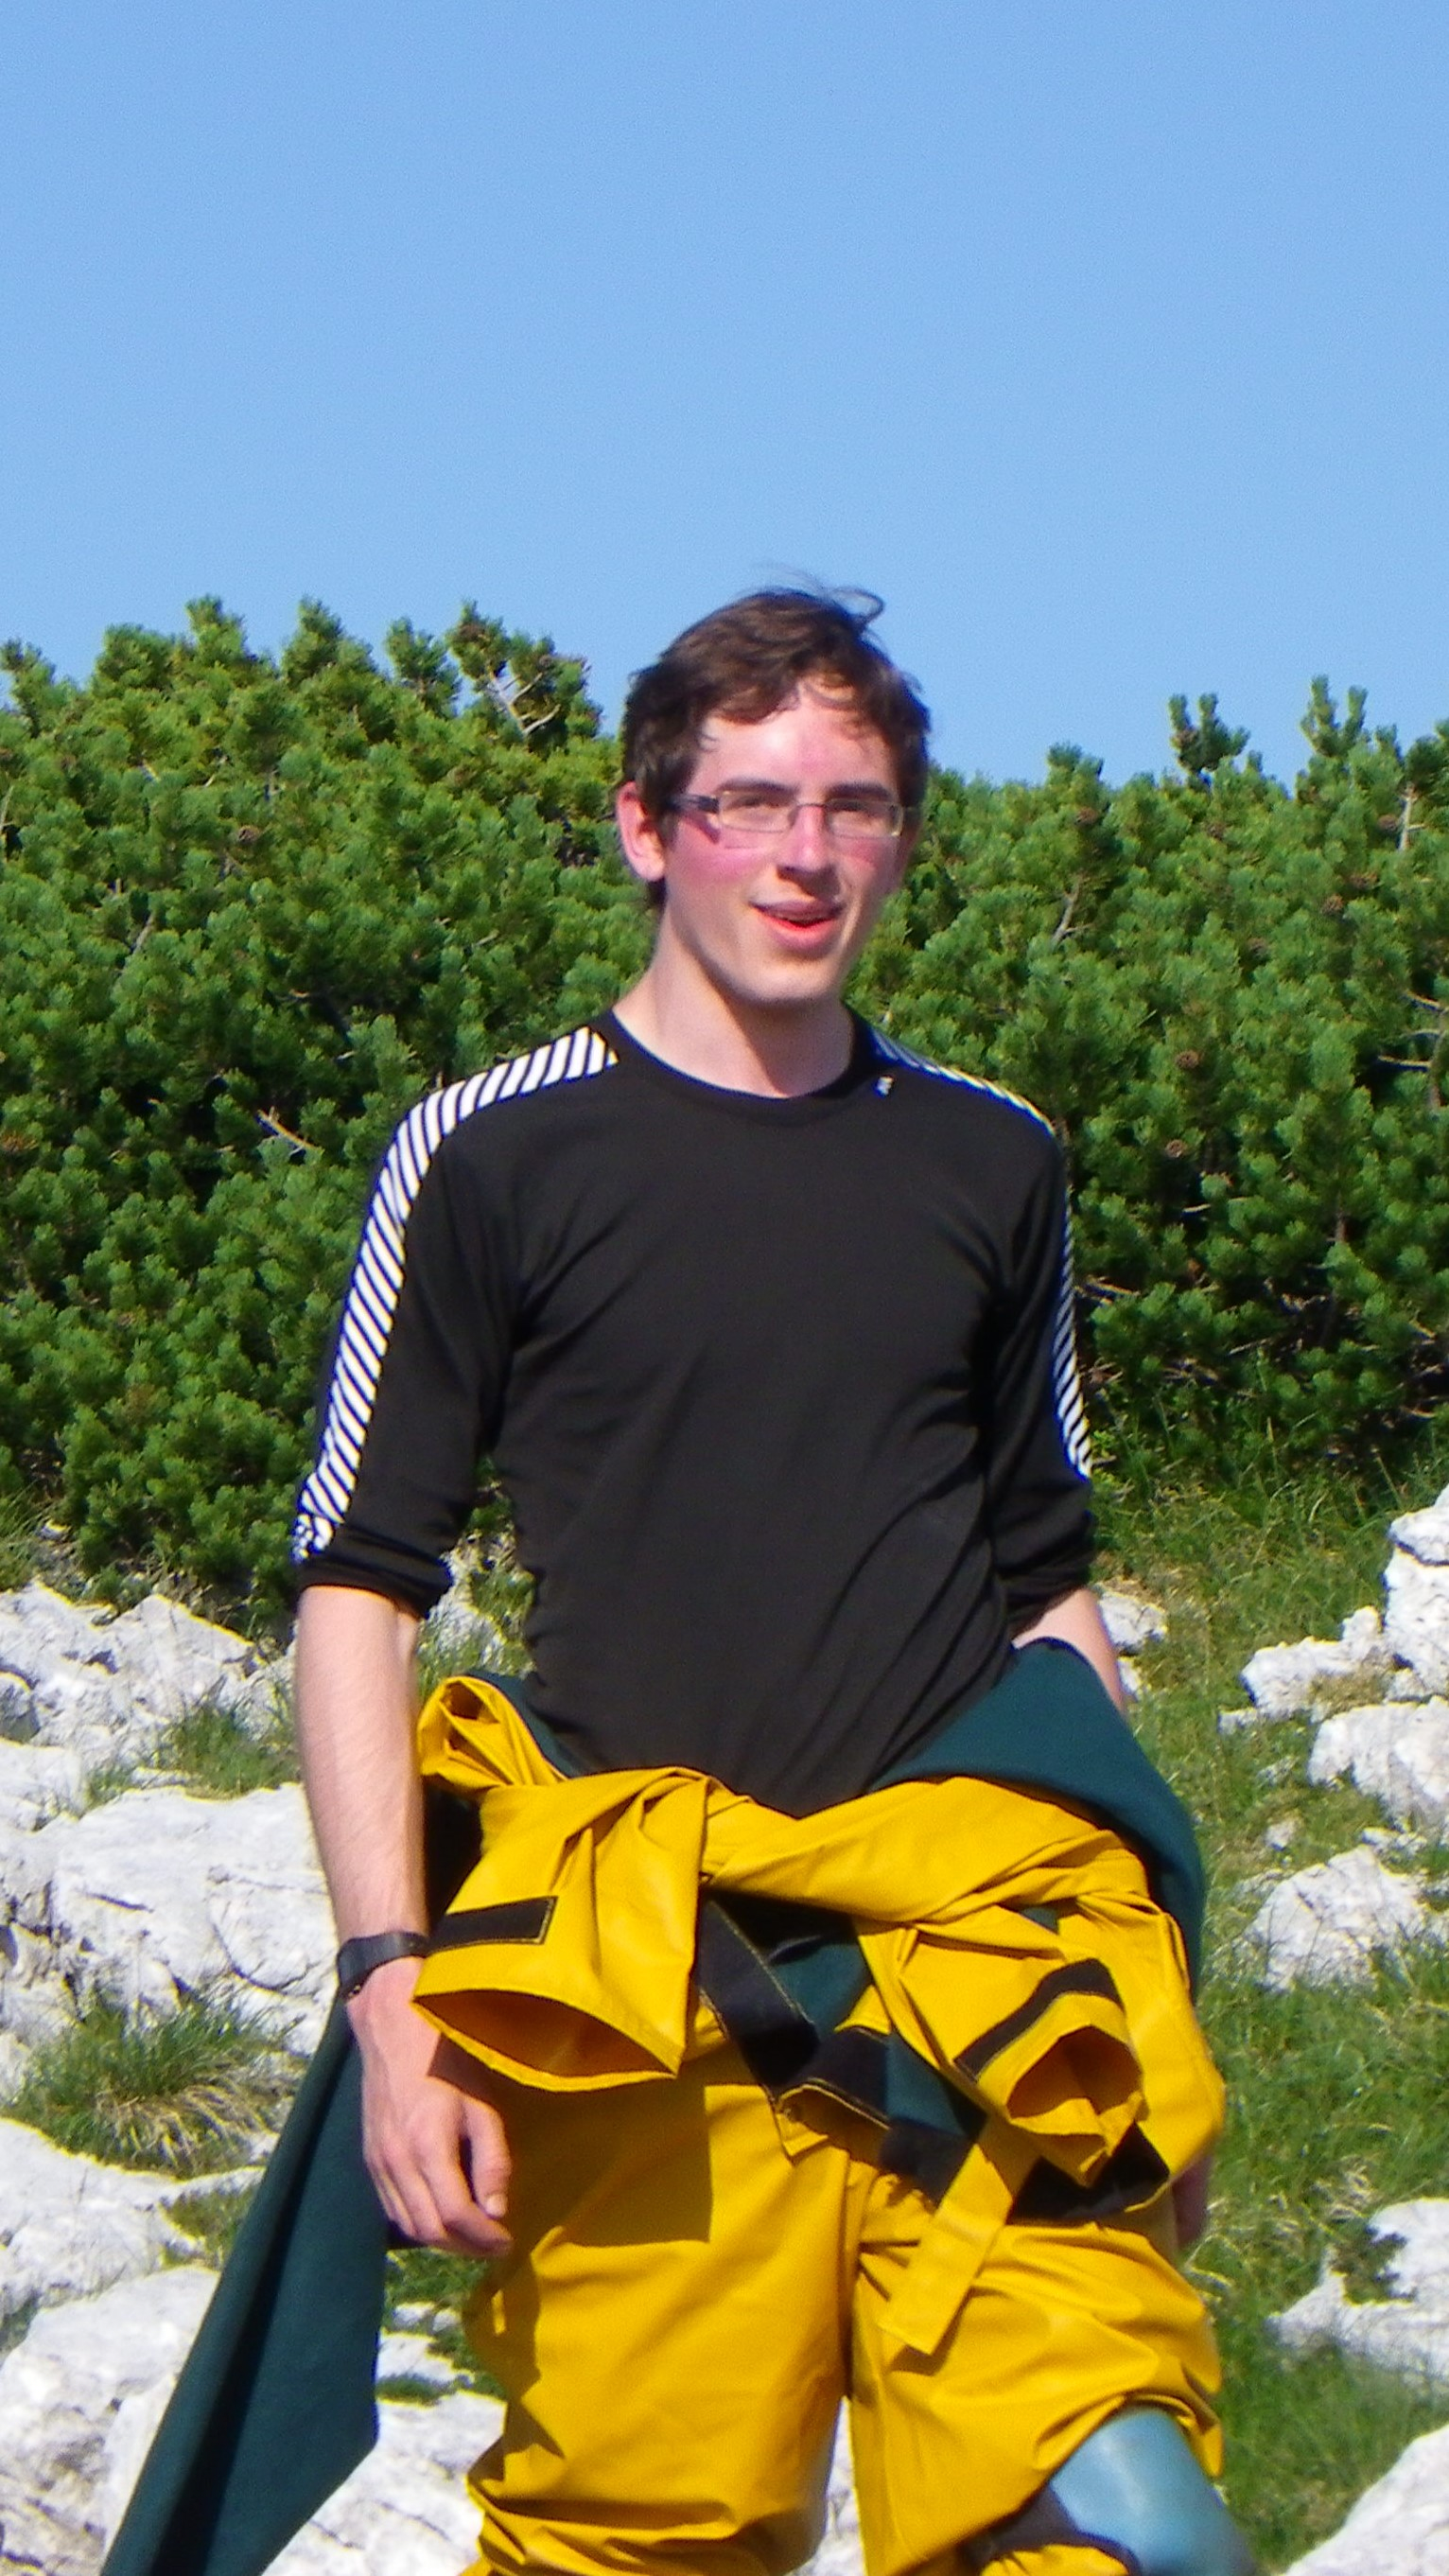
\includegraphics[width=\linewidth]{2012/hotpants/2012-07-18-18.44.08-Rhys Tyers-Pentax X90-IMGP3303--orig.jpg}} 
 \caption{Oliver Myerscough ready to join the underground camp set-up trip. Clare and Jarv would discover \passage{Watership Down} a couple of days afterwards; Oli would later find \passage{Watership Up} with Jarv. \pic{Rhys Tyers}}
 \label{oli caving}
\end{marginfigure}

A smooth trip down to \passage{Red Cow} was had, just enough of the route
memorised from last year to make it smooth. We discussed the camping
potential at \passage{Red Cow} (very pleasant, I think) and despaired at the (lack
of) quality in the rigging on the many little climbs and occasional
pitches from the bottom of \passage{Big Rock Candy Mountain}. ``On behalf of the entire 2003 \&
2004 expedition I apologise'' spoke Tetley on a previous trip with
Clare.

I was interested in checking out the `downstream' sump at \passage{Red Cow}, which
takes the majority of the water from the \passage{Republica} chamber. So we
followed a few cascades and reached a 3 metre drop with a single bolt. I
believe the survey starts around here, but it's difficult to say as this
region is poorly PSS. We attached one of our ropes, I abseiled down
managing to walk back in the chamber to avoid the waterfall. The lake at
the bottom of this chamber was not in fact the sump, rather a metre wide
phreatic tube led off for perhaps ten metres, finally reaching a bend
where the roof continued dipping but the water stayed still and level,
with pools of brown silt sitting in the otherwise pure white floor.

\margininbox{Perfidia}{
     \begin{itemize}
    \item Jarvist Frost
    \item Clare Tan
    \end{itemize}}{\explo}

Derigged, we climbed up in the rift at the previous cascade, and found
an obvious dry level. This was strange, as I knew this passage was not
on the survey, but there were clear marks from cavers passing. Clare and
I decided to give it a proper push. Soon we found ourselves discarding
bits of SRT kit and harness. We made a good team, Clare wriggling off
through the smallest of gaps while I continued to expand them to human
size behind. A flat out squeeze over cobbles took a while to reengineer,
and a ninety degree bend to stand up in a wriggle rift took a lot of
hammering by Clare to make it passable. Alas, she found herself in a
region, again, with obvious caver marks the far side of the tight stuff,
and soon said, ``I've been here before,'' as she found a \passage{Republica} PSS. We had
connected between the downstream \passage{Red Cow} sump and the head of
\passage{Insomnia} pitch (climb back out across the pitch along the large
ledges, before turning right into a chamber leading off), connecting the
`crescent' shown previously on the survey. 

\margininbox{21/7/2012 6:57 pm}{
 Excellent push
yesterday, even if everything we found (\textasciitilde 150 m total?)
seemed to be body-sized or smaller!

\passage{Perfidia} is a cool connection between \passage{Red Cow} (pitch rope) and the start
of \passage{Insomnia}. Saves a fair bit of time, though only go there if
you aren't carrying lots of tackle and are shorter than Jarv! \name{Clare}}{\logbook}

This only further complicates
our understanding of the hydrology here -- was this the old route for
the \passage{Red Cow} water, did it join up at \passage{Insomnia} to form that
impressive pitch, before it found a way out through the present cascades
and sump? Still, we had fifty-five metres of survey in the book, a good
thirty of which were new, where many cavers must have stood but none
decided to push. This also offers a tight, though not horrifically so,
flood safe bypass for \passage{Republica}. With further enlargement it could even
become the through way.

So, after a couple of hours diversion, we continued to our main target
-- the bottom. \passage{Insomnia}'s rope was badly hung up, I had to
reverse prussic about 20 m directly through the water before I'd
stretched enough slack to rig my descender and very very gently
(checking the rope) descended \& unhooked the rope from the crack it had
been wedged in.

The wet ropes in \passage{Insomnia} were found to be in good nick, and so
we abandoned the rigging gear to speed our progress. Interestingly, the
only place where the rope had been abraded was the natural tied off bit
to help you avoid landing in the big pool. Here the rope had been
dangling a natural `L' shape, and being gently swung back and forwards
by the draught had sliced through the sheath and most of the core where
it touched the rock ridges on the floor.

\margininbox{Watership Down}{
     \begin{itemize}
    \item Jarvist Frost
    \item Clare Tan
    \end{itemize}}{\explo}

Back at \passage{Winter Journey}, we threw ourselves into the rift and soon
reached the exploration end. I essentially pushed Clare into the rift
taking the draught, and she started enlarging with the bolting hammer
and squeezing away. Progress was pretty quick, but I was captivated by
the inclined bedding plane leading off. By myself, I hadn't dared climb
down this last year. It didn't look so bad now, and Clare would
definitely be able to follow me into this `lobster pot' if that's what
it turned out to be.

So I slithered down and away, a pretty long way down over dried silt,
and reached a crawl way at the bottom. There was a gentle draught once
more. I called Clare down, though she had nearly made it through her
upward squeeze. We padded off through the rabbit warren like passage,
dull thuds of our paws on the soft floor. ``\passage{Watership Down}'' was
the obvious name for this find -- especially as I knew Clare liked the
book. A branch to the right led upwards to a pitch into a chamber.
Continuing ahead entered a slightly more confined space and a crawlway
climbing back up the bedding to reach a T-junction. Here a large draught
blew across, coming from a crawl / stoop leading down from the right.
The way to the left soon turned into an inclined rift climb, steeper
than other bits of bedding had seemed. But it was negotiable with
care. The next climb looked rather more committing, the walls clearly
belling out into a proper chamber, and what was that dark space down
there?

I must admit exploration fever had rather got me at this point, as \bignote{I
climbed down without much concern for the return journey}. 

I was
stunned by what I climbed down towards -- a large, crystal clear, sump
with an underwater rock arch leading off into turquoise blue depths. 
A fridge sized boulder sat on the white sandy beach, which then seemed to descend steeply underwater (perhaps 45 degrees), with another large boulder sitting underwater. 
The water was crystal clear, and between the boulder on the floor and the rock arch was a deep deep blue. 
The rift had widened to about 3 m at this point, and the sump pool was perhaps 4 m deep. 

The
seriousness of our situation was underlined by Clare's arrival, with \bignote{a clatter and a whoosh as she lost her footing} and nearly,
in that caving cliché, fell into the terminal sump.

We ignored the cliff-face that was our only way out, and continued
exploration. The main sump was beautiful, but a parallel route through
the boulders led to a smaller, obviously connected, body of water. A balcony was visible on the other side of the main sump, and with a rope,
would be a passable pendulum. 


\margininbox{Herman Herz, 2013}{Clare Tan for a narrow escape in Slovenia. During the 2012 summer expedition, whilst pushing the deepest part of the cave (nearly 1km below the surface), Clare and Jarv made a breakthrough into a steep climb down a widening rift. Jarv managed to climb down the $\approx$50 degree slope before Clare arrived at the bottom at speed, having slipped down. After exploring the new found sump pool, their one mission was to escape.}{\award}

Feeding into the sump was a dry inlet,
which led away through a small crawlway, forming part of the rift we had climbed down. 
This we pushed up until it started
to get rather catchy and surveyed out, though further progress is
certainly possible. 
By this point the sump was slowly starting to fill with white smoke, as our motion fed rock-flour into the sump. 
Our survey at sump level complete, including a plastic
PSS at the exact water level on the sandy beach, we had to tackle the climb and attempt our escape. 

Clare
went up first, after a few false starts and slithering back down, we
found a working method utilising `combined tactics', where I would
bridge across the floor and ceiling and be stood on. Her safely up, I
slipped back down again and was lowered the end of the survey tape to
complete the measurements -- 9.83 m to safety.

There was \bignote{nothing Clare could do to help} as I slipped and struggled. The
mud on the walls had been made slimy, the footholds were degenerating. I
slowly slithered up the far end of the rift where it was narrow and I
could bridge most effectively, but therefore had to deal with
overhanging sections which I scaled, somehow, with the minimum of poise
and grace. As we surveyed out Clare had to indicate the stations again
and again, the buzzing in my head was dissolving memories as fast as
they were forming.

Time was pressing on and we did not have time to look at the many leads
left in the rabbit warrens. Instead we made a speedy exit, Clare taking
the exploration bits and bobs, I choosing to pull up the ropes as there
is never a guarantee of return at these extreme ends of the cave system.

\tweet{8:14AM Jul 23, 2012}{First explo team out.VRTNARIJA almost certainly below 900m with WATERSHIP DOWN leading from WINTER JOURNEY to beautiful crystal clear sump.}

\passage{Red Cow} offered its usual calming influence; the strange `quiet
corridor in an alien spaceship' feel to these horizontal sections was
now comforting where it had previously been disquieting. We sat there munching the food
we had stashed on the way in, rehydrating even as our Meander oversuits
steamed off their splashes from \passage{Insomnia} and \passage{Republica}. I thought \bignote{dark thoughts about the riggers} of both these pitches, in their
different `exploration rigging' ways my two most hated and, in my
consideration, dangerous pitches of the cave. And there they were
together, back to back, a gauntlet to be passed on the way to the
depths, and a horrible back-of-mind barrier to the exit to safety.

The way back to camp passed smoothly. Back for tea and medals, talk of
daring do and plans for a rather more sedate second day.


\subsection{The Day After}

\margininbox{Hot Pants}{
     \begin{itemize}
    \item Jarvist Frost
    \item Clare Tan
    \end{itemize}}{\explo}

Our plan for the second day was rather more constructivist in intent.
Since exploring the \passage{Throne Room} last year, no one had returned
except to the large obvious windows which had formed `\passage{Amazing
Grace}' and the way to the East. Clare and I knew there to be a
potential traverse, and also a short pitch. This area is relatively
close to Camp \passage{X-Ray} and so would be a good place for less
experienced teams to cut their exploration teeth. So we packed up the Uneo drill and
made our way along \passage{Kamikaze} and the \passage{Red Baron} traverse. The leads are as
we remember them, and I quickly rig up the start of the traverse and
place a bolt in the large boulder for abseil (with tackle sac rope
protector) into the pit. Confirming it's a going lead with a pitch
leading off, I come back up and get stuck into the main metal of the
traverse\sidenote{Nico et al. dropped this pitch, and a few more climbs and cascades before it degenerated -- from the survey and form of the cave, it looks as if you're descending the immature vadose formation below the \passage{Throne Room} boulder
collapse.}.


The first few bolts are just fine -- swing and bolt, rejiggle the
rigging and move outwards one metre. From my perch around the corner, I
realise that this is rather more demanding than had been hoped -- not a
traverse over the pit and into a side passage, but a continuing climb
traverse out of the end of the chamber. I keep at it, finding passable
rock to bolt in the overhung ceiling, and somehow climbing backwards
over stopped boulders and chunks of dried mud. I am not, as it were,
enjoying myself at this point. The bolts aren't being tested as I pass,
and I'm climbing a good few metres in height between placements, on semi
static rope and without a belayer, just judging the length of slack.
Considerable quantities of footholds disappear bouncing down the slope,
flying into the pit at the bottom. I explain this predicament to Clare.
She replies with ``Well, you don't have any choice -- we don't have the
dynamic rope with us and we're not going back to camp.'' Charmed.

Clare, shivering on a boulder while I sweated with outstretched drill,
also has an idea for the survey name -- \passage{Hot Pants}. Why? ``I have a plan,
and it's as hot as my pants\ldots{}'' - Lord Flashart

At the top I reach a little chamber with an obvious climb leading up
through a boulder choke. The traverse rope is just long enough to belay
as far as the top of the climb, but not to protect the way across.
Feeling rather flushed and vertiginous at the achievement (19.44 m at 50
degrees says the survey, between here and the last traverse bolt) I
finalise the rigging. Clare follows me on the rigged line, I watch it
scratch at a particularly large pile of boulders which I didn't dare
disturb -- derigging from the bottom and gardening back from the top
would make a lot of sense long term.

We climbed up carefully through the boulder choke and were rewarded with
a beautiful little chamber, about 12 x 4 m, with a high ceiling and an
obvious balcony a good four metres off the floor. Out of tackle, we looked
at the crawlway heading NNW out of the chamber. This was taking a
distinct draught, and was easy (though rather small) going with a white
silt floor. Clare slithered over a little dam and wriggled off, coming
back to state it was going but rather small. I couldn't be bothered with
such arduous squeezing at this stage, and expecting that this lead would
be looked at first before bolt climbing plans, was happy to survey out.

[Strangely, this crawl wasn't again looked at -- instead the teams who
came after us hand bolt climbed to the balcony and beyond, gaining
passage 7 metres above the chamber floor, which led to 73 m of gently
descending passage to the NNE (\passage{Peep Show}), terminating at a boulder
choke, and then 78 m of gently ascending passage due North into blank
mountain (\passage{Undercover Squirrel}) terminating at a 4 m draughting climb
into a chamber.]

\margininbox{22/7/12 9:01}{Really should be asleep, but am just on the wrong side of restless to do
so! Fingers crossed the day train doesn't arrive to kick us out of
bed\ldots{} Rhys has just got up for a piss, only to find the piss BDH
full\ldots{} so he promptly went to \passage{Zimmer} to empty it. What a
trooper! \name{Clare}}{\logbook}


And that was the story of my first camping trip with Clare. I certainly
felt rather pleased -- we had gone after the lesser leads and multiplied
them through our efforts. Finding the beautiful \passage{Watership Down}
sump was a joy, but the \passage{Hot Pants} traverse climb was perhaps the most
important work in terms of the exploration it enabled.

\name{Jarvist Moore Frost}